\begin{figure}[H]\centering
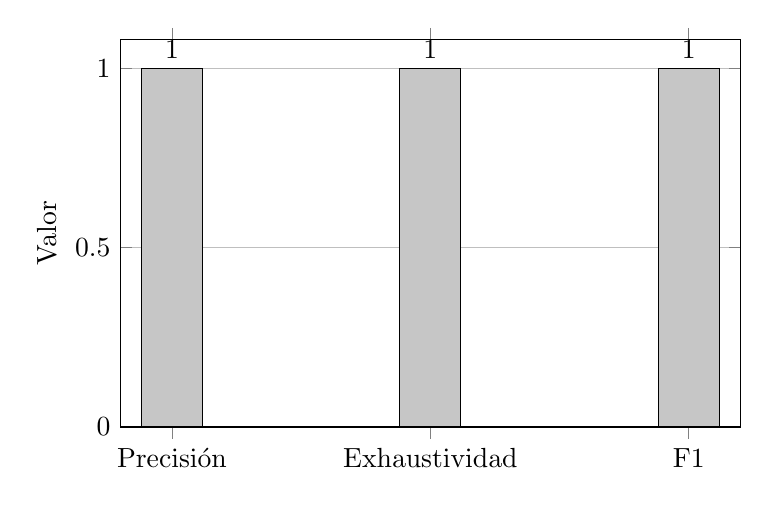
\begin{tikzpicture}\begin{axis}[ybar,bar width=22pt,width=.78\textwidth,height=6.5cm,ymin=0,ymax=1.08,ylabel={Valor},symbolic x coords={Precisión,Exhaustividad,F1},xtick=data,ymajorgrids=true,nodes near coords]
\addplot[fill=gray!45,draw=black] coordinates {(Precisión,1.0) (Exhaustividad,1.0) (F1,1.0)};\end{axis}\end{tikzpicture}
\caption{Contratos sintéticos de recuperación en 30 repeticiones. No constituyen evaluación humana de un modelo generativo.}\label{fig:contratos-ia}\end{figure}
